\section{Experimential results}
\label{sec:results}

This work does not only proposes three new methods to realize collision
avoidance in dynamic environments with \ac{fabrics}, but it also includes an
analysis of the different methods under noisy sensor data. In the real world, 
sensor data, but also the perception pipeline detecting obstacles and occupied
voxels, produces sensor noise. In this section, we present quantative
comparisons for three simulation environments, namely a holonomic ground robot,
a non-holonomic ground robot and a robot manipulator. For all cases, we evaluate
50 cases with different noise levels $\sigma$. The noisy signal is generated
using a Gaussian distrubtion centered around the unoisy sensor data. 
The performance is measured 
in terms of sucess, solver time and execution time to reach the goal. Lastly, 
we evaluate the methods in the real world using a real manipulator.

\begin{figure}
  \begin{subfigure}{0.5\linewidth}
    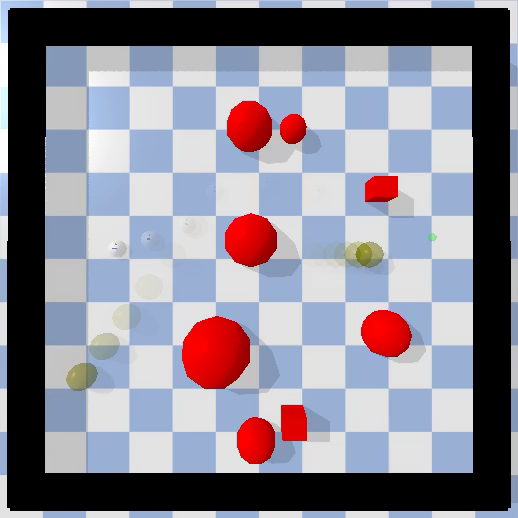
\includegraphics[width=0.95\linewidth]{point_robot_sim/case}
    \caption{Point Robot Case}
    \label{fig:point_robot_case}
  \end{subfigure}%
  \begin{subfigure}{0.5\linewidth}
    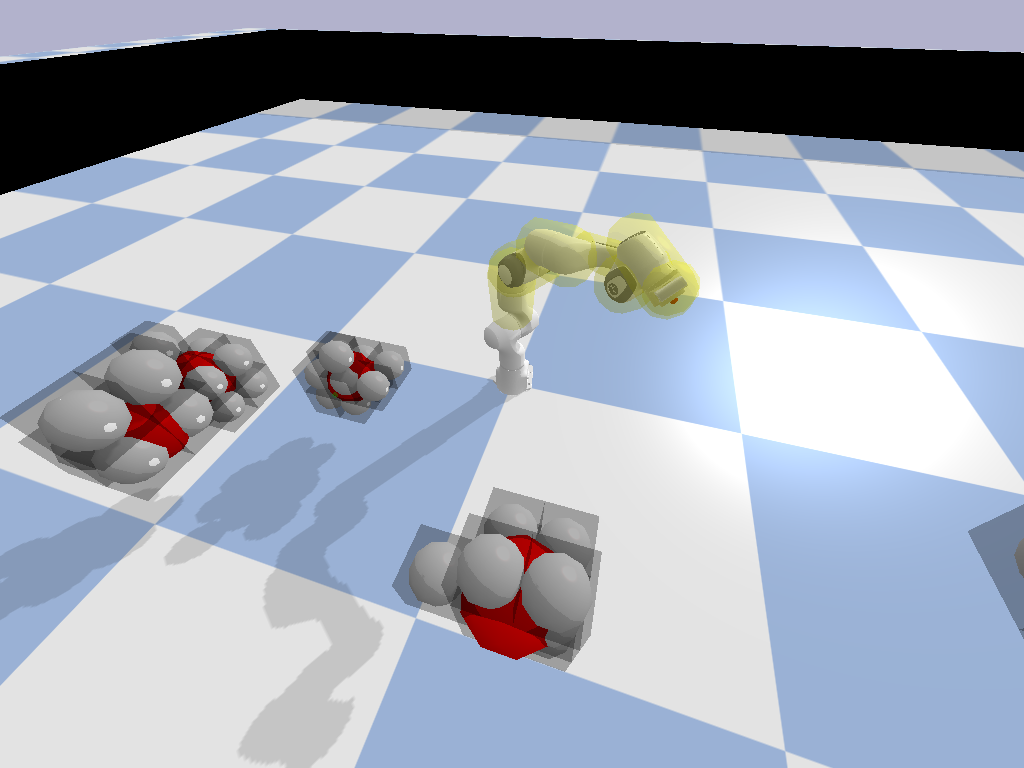
\includegraphics[width=0.95\textwidth]{methods/raw_sensors_panda.png}
    \caption{Occupancy Grid}
    \label{fig:panda_raw_sensors}
  \end{subfigure}%
\end{figure}


\paragraph{Details on implementation}
The planner's implementation can be found at
\href{www.github.com/tud-amr/fabrics}{Geometric Fabrics}. The simulation
environment as well as the the algorithm for computing the \ac{fsd}, \ac{sdf}
and the raw lidar data can be found as part of
\href{www.github.com/maxspahn/gym_envs_urdf}{urdfenvs}. For the real world
experiments, we used a ros bridge and used the same
implementation to process the real point cloud generated by
a highly reactive octomap \cite{Hornung2013}.

\subsection{Point Robot}
\label{sub:point_robot}

When comparing explicit environment representations with the proposed techniques
using noise-free sensor data ($\sigma=0.0$), \acp{sdf} demonstrate the highest
success rate. This is likely due to the \textit{guidance} provided by the
\ac{sdf}'s gradient information. However, intriguingly, the explicit method's
performance appears to improve with increasing noise ($\sigma$), warranting
further investigation.

The goal reaching times remain similar across all approaches, which aligns with
expectations as the tuning is based on this criterion, as shown in
\cref{subfig:point_robot_sim_time2Goal}. While solver computation times are low
for all methods (approximately $3.5$ ms), utilizing raw lidar data substantially
increases computational costs, as observed in
\cref{subfig:point_robot_sim_solvertimes}. This increase results from accounting
for a greater number of obstacles compared to the other methods.


\begin{figure}[h]
  \centering
  \begin{subfigure}{0.33\linewidth}
    \centering
  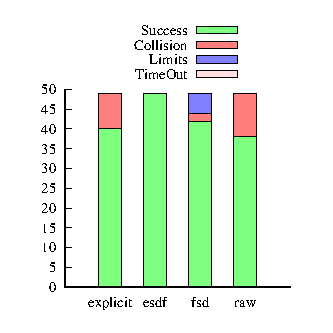
\includegraphics[width=1.0\textwidth]{point_robot_sim/success_PointRobot_00}
    \caption{$\sigma = 0.0$}%
    \label{subfig:point_robot_sim_sucess_noise_00}
  \end{subfigure}%
  \begin{subfigure}{0.33\linewidth}
    \centering
    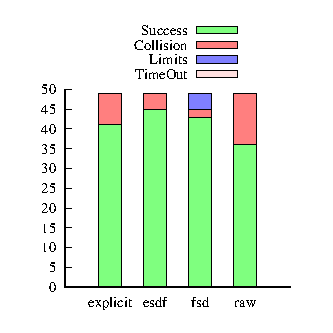
\includegraphics[width=1.0\textwidth]{point_robot_sim/success_PointRobot_01}
    \caption{$\sigma=0.1$}%
    \label{subfig:point_robot_sim_success_noise_01}
  \end{subfigure}%
  \begin{subfigure}{0.33\linewidth}
    \centering
    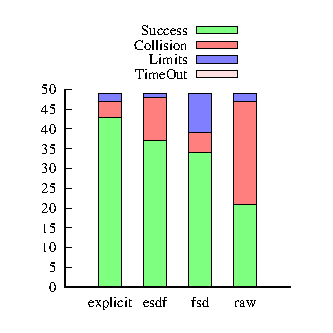
\includegraphics[width=1.0\textwidth]{point_robot_sim/success_PointRobot_02}
    \caption{$\sigma=0.2$}%
    \label{subfig:point_robot_sim_success_noise_02}
  \end{subfigure}%
  \caption{Point robot in simulation.
  }%
  \label{fig:point_robot_sim_success}
\end{figure}

\begin{figure}[h]
  \centering
  \begin{subfigure}{0.5\linewidth}
    \centering
  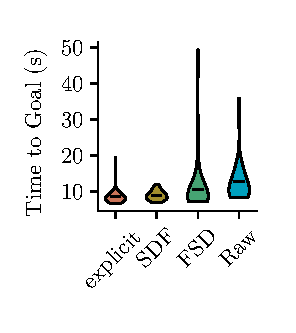
\includegraphics[width=0.9\textwidth]{point_robot_sim/time2Goal_PointRobot_00}
    \caption{Goal reaching time}%
    \label{subfig:point_robot_sim_time2Goal}
  \end{subfigure}%
  \begin{subfigure}{0.5\linewidth}
    \centering
    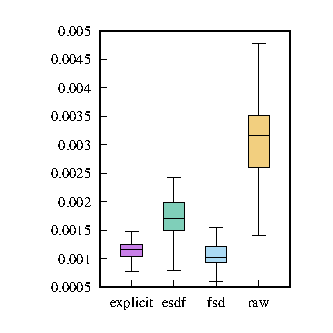
\includegraphics[width=0.9\textwidth]{point_robot_sim/solvertime_PointRobot_00}
    \caption{Solvertimes}%
    \label{subfig:point_robot_sim_solvertimes}
  \end{subfigure}%
  \caption{Point robot in simulation.
  }%
  \label{fig:point_robot_sim_metrics}
\end{figure}

\subsection{Panda}
\label{sub:panda}

When examining results obtained with the \ac{panda} robot, there is a notably
greater variance in performance compared to those observed with the point robot.
Notably, it becomes evident that \ac{fabrics} exhibit heightened robustness in
dynamic environments marked by noisy sensor data, particularly when employing
\ac{fsd}. This approach maintains a high success rate as noise levels escalate,
in contrast to the significant performance degradation observed with other
methodologies, as depicted in \cref{fig:panda_sim_success}.

Furthermore, \ac{fsd} boasts the shortest computational times, approximately $1$
ms. This underpins the conclusion that in dynamic settings, \ac{fsd} harmonizes
most effectively with the \ac{fabrics} framework. This finding aligns with
outcomes from receding horizon optimization techniques, such as those
highlighted in \cite{Tordesillas2019}, applied to \ac{mpc} formulations
involving drones.

\begin{figure}[h]
  \centering
  \begin{subfigure}{0.33\linewidth}
    \centering
    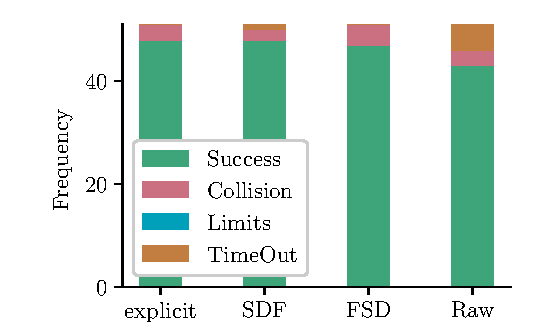
\includegraphics[width=1.0\textwidth]{panda_sim/success_Panda_00.eps}
    \caption{$\sigma = 0.0$}%
    \label{subfig:point_robot_sim_sucess_noise_00}
  \end{subfigure}%
  \begin{subfigure}{0.33\linewidth}
    \centering
    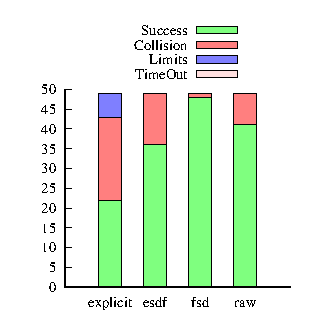
\includegraphics[width=1.0\textwidth]{panda_sim/success_Panda_005.eps}
    \caption{$\sigma=0.05$}%
    \label{subfig:panda_sim_success_noise_005}
  \end{subfigure}%
  \begin{subfigure}{0.33\linewidth}
    \centering
    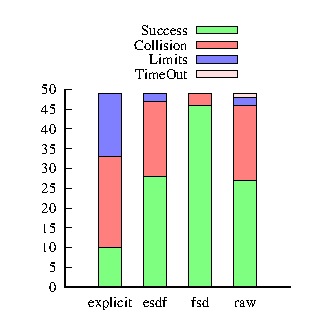
\includegraphics[width=1.0\textwidth]{panda_sim/success_Panda_01.eps}
    \caption{$\sigma=0.1$}%
    \label{subfig:panda_sim_success_noise_01}
  \end{subfigure}%
  \caption{Panda robot in simulation.
  }%
  \label{fig:panda_sim_success}
\end{figure}

\begin{figure}[h]
  \centering
  \begin{subfigure}{0.5\linewidth}
    \centering
  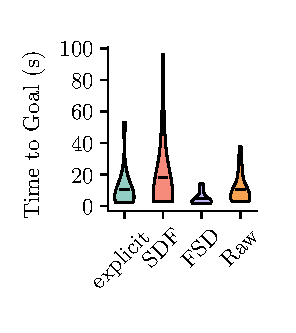
\includegraphics[width=0.9\textwidth]{panda_sim/time2Goal_Panda_00}
    \caption{Goal reaching time}%
    \label{subfig:panad_sim_time2Goal}
  \end{subfigure}%
  \begin{subfigure}{0.5\linewidth}
    \centering
    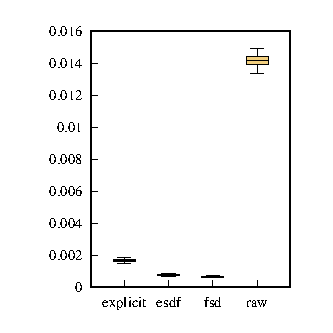
\includegraphics[width=0.9\textwidth]{panda_sim/solvertime_Panda_00}
    \caption{Solvertimes}%
    \label{subfig:panad_sim_solvertimes}
  \end{subfigure}%
  \caption{Panda robot in simulation.
  }%
  \label{fig:panad_sim_metrics}
\end{figure}

\subsection{Real-World Experiments} % (fold)
\label{sub:real_world_experiments}


